\documentclass{article}
\usepackage{CJKutf8}
\usepackage{indentfirst}
\usepackage{graphics}
\usepackage{epsfig}
\usepackage{graphicx}
\usepackage{amsmath}
\usepackage{amssymb}
\usepackage{listings}
\usepackage{tikz}
\usetikzlibrary{matrix,chains,positioning,decorations.pathreplacing,arrows,calc}
\usepackage{algorithmic}
\usepackage{algorithm}

\setlength{\parindent}{2em}
\renewcommand{\contentsname}{目录}
\renewcommand{\listfigurename}{插图目录}
\renewcommand{\listtablename}{表格目录}
\renewcommand{\refname}{参考文献}
\renewcommand{\abstractname}{摘要}
\renewcommand{\indexname}{索引}
\renewcommand{\tablename}{表}
\renewcommand{\figurename}{图}

\makeatletter
\newcommand{\HEADER}[1]{\ALC@it\underline{\textsc{#1}}\begin{ALC@g}}
	\newcommand{\ENDHEADER}{\end{ALC@g}}
\makeatother
%opening
\date{2016年11月}
\title{基于神经网络的sin函数拟合实验报告}
\author{何宜晖\\计算机46\\2140504137}
%\\heyihui@stu.xjtu.edu.cn
\begin{document}
\begin{CJK}{UTF8}{gkai}
%gkai gbsn
\begin{figure}
\centering

\includegraphics[width=0.6\linewidth]{xjtu}
\end{figure}


\maketitle
\clearpage
\section{实验内容}
利用两层神经网络,拟合sin函数。
\section{实验目的}
人工神经网络是近年来发展起来的模拟人脑生物过程的人工智能技术,具有自学习、自组织、自适应和很强的非线性映射能力。在人工神经网络的实际应用中,常采用BP神经网络或它的变化形式,BP神经网络是一种多层神经网络,因采用BP算法而得名,主要应用于模式识别和分类、函数逼近、数据压缩等领域 \cite{bao2010} 。  

本次实验利用BP网络修改权值对$y=sin(x)$曲线实现拟合,并比较了各种实现细节。

\section{实验原理}
传统的感知器和线性神经网络不能解决非线性问题,因此在实际应用过程中受到了很大的限制。

BP网络是一种多层前馈神经网络,由输入层、隐层和输出层组成。层与层之间采用全互连方式,同一层之间不存在相互连接,隐层可以有一个或多个。
BP算法的学习过程,主要有两个阶段,由前向计算过程和误差反向传播过程组成,
在前向计算过程中,输入信息从输入层经隐层逐层计算,并传向输出层,每层神经元的状态只影响下一层神经元的状态。
在反向计算过程中,误差信号沿原来的传播路线返回,通过修改各层的权值,使得网络系统误差下降,最终实现函数的拟合。

反向传播算法,在算法1中详细描述。

\begin{algorithm}\label{algo}
	\caption{反向传播算法}
	\begin{algorithmic}
		\FOR{样本 in 数据集}
		\HEADER{前向传播}
		\STATE 从第一层开始,计算每一层的激活
		\ENDHEADER
		\HEADER{反向传播}
		\STATE 计算每一层对于误差的导数
		\FOR{层 in 所有层}
		\STATE 计算误差对于本层权值的导数
		\STATE 计算误差对于下一层的导数
		\ENDFOR
		\STATE 更新权值
		\ENDHEADER
		\ENDFOR
	\end{algorithmic}
\end{algorithm}

在本实验中,输入层只有一个单元x,输出层只有一个单元y,神经网络的结构如图1所示。
\tikzset{%
	every neuron/.style={
		circle,
		draw,
		minimum size=1cm
	},
	neuron missing/.style={
		draw=none, 
		scale=4,
		text height=0.333cm,
		execute at begin node=\color{black}$\vdots$
	},
}
\begin{figure}
	\centering
	\begin{tikzpicture}[x=1.5cm, y=1.5cm, >=stealth]
	
	\foreach \m/\l [count=\y] in {1}
	\node [every neuron/.try, neuron \m/.try] (input-\m) at (0,1-\y) {};
	
	\foreach \m [count=\y] in {1,missing,2}
	\node [every neuron/.try, neuron \m/.try ] (hidden-\m) at (2,2-\y*1.25) {};
	
	\foreach \m [count=\y] in {1}
	\node [every neuron/.try, neuron \m/.try ] (output-\m) at (4,1-\y) {};
	
	\foreach \l [count=\i] in {1}
	\draw [<-] (input-\i) -- ++(-1,0)
	node [above, midway] {输入$I$};
	
	\foreach \l [count=\i] in {1,n}
	\node [above] at (hidden-\i.north) {隐层单元$H_\l$};
	
	\foreach \l [count=\i] in {1}
	\draw [->] (output-\i) -- ++(1,0)
	node [above, midway] {输出$O$};
	
	\foreach \i in {1}
	\foreach \j in {1,...,2}
	\draw [->] (input-\i) -- (hidden-\j);
	
	\foreach \i in {1,...,2}
	\foreach \j in {1}
	\draw [->] (hidden-\i) -- (output-\j);
	
	\foreach \l [count=\x from 0] in {输入层, 隐含层, 输出层}
	\node [align=center, above] at (\x*2,2) {\l };
	
	\end{tikzpicture}
		\label{fig:neural}
	\caption{神经网络结构}
\end{figure}
 

\section{具体实现}
\subsection{数据准备}
要对BP网络进行训练,必须准备训练样本。对样本数据的获取,可以通过用元素列表直接输入、创建数据文件,从数据文件中读取等方式,具体采用哪种方法,取决于数据的多少,数据文件的格式等。  本使用均匀分布在线生成100个训练样本,以及100个测试样本。同时采用归一化处理,使得 $x \in [-1, 1], y\in [-1, 1]$。归一化后的训练样本如下图:

\begin{figure}
	\centering
	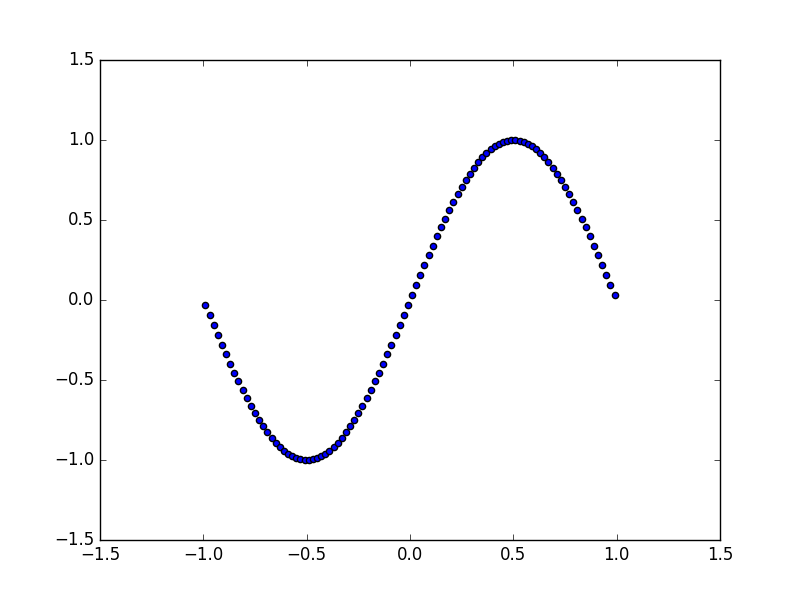
\includegraphics[width=\linewidth]{../scatter}
	\caption{训练集}
	\label{fig:fig0}
\end{figure}
\subsection{参数设定}
根据系统输入输出序列,确定网络输入层节点数为1,
隐含层节点数H为10,(根据经验公式,$N_H = N_{samples}/10$ ),
输出层节点数为1。初始化输入层、隐含层和输出层神经元之间的连接权值\cite{he2015delving}
\begin{equation}
	w_{l+1} = N(0,\sqrt{2/\hat{n_l}})
\end{equation}
其中$n_l$为前一层神经元个数, $l$为层数,

给定学习速率 $10^{-2}$, 给定算法迭代次数100000,同时给定神经元激励函数tanh。

激励函数,可设置为多种形式,本实验中所选函数为$tanh$,从直觉讲,它的曲线较为平滑,输出在-1到1, 更利于正弦正弦函数拟合, 如图\ref{fig:tanh}:
\begin{equation}
	tanh(x) = \frac{e^{2x}-1}{e^{2x}+1}
\end{equation}
\begin{figure}
	\centering
	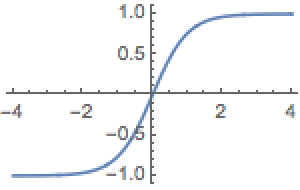
\includegraphics[width=.3\linewidth]{../tanh}
	\caption{tanh}
	\label{fig:tanh}
\end{figure}

\subsection{BP算法实现的正确性检测}
以上我们叙述了神经网络的实现细节, 在开始实验前,还需要做一点就是:梯度检查。保证算法实现的正确性,我们采用下面的相对误差判断法, 首先计算真实梯度A,我们令BP算法计算的梯度为B:
\begin{equation}
	A = \frac{f(x+\Delta x)-f(x-\Delta x)}{2\Delta x}
\end{equation}
\begin{equation}
\frac{|A-B|}{max(10^{-8}, |A+B|)} < \delta
\end{equation}
其中,$\delta$取$10^{-7}$. 经过检查,我的相对误差在$10^{-9}$, 检查通过,可以安全地进行进一步实验。

\subsection{初步拟合}
我们简单设置了参数,初步拟合sin函数,如图\ref{fig:fig1}.
我们使用MSE作为我们的误差评判标准:
\begin{equation}
	MSE = \frac{1}{n}\sum_{n}^{k=0}(y-f(x_k))^2
\end{equation}
初步拟合的误差为$10^{-3}$,可以看出,拟合的效果并不好。

\begin{figure}
\centering
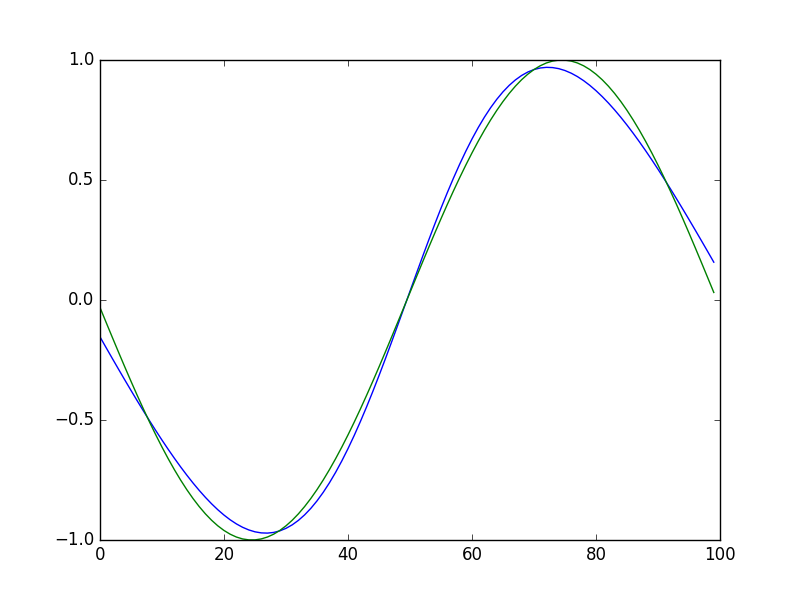
\includegraphics[width=.8\linewidth]{../fig1}
\caption{初步拟合(测试集)}
\label{fig:fig1}
\end{figure}

\subsection{过度拟合问题}
实验中发现,当隐含层单元较多时,比如100,会有一定程度的过度拟合,
而我们根据经验公式选择的10个单元,不会发生过度拟合。

\subsection{算法改进}
为了进一步提高拟合的准确率,我们作出了两点改进。
学习率的改进,不再采用固定学习率,而采用阶梯学习率

\begin{equation}
	lr = lr_0  \gamma^{[\frac{iter}{step}]}
\end{equation}
其中$lr0$ 为初始学习率,iter为目前迭代次数,$\gamma$为衰减系数,$step$为一个阶梯的迭代次数。我们一共设置3个阶梯。

另外,我们将神经网络开始到结束每次迭代的结果,用指数衰减结合起来\cite{karpathy2016cs231n}。
\begin{equation}
W^k_{ij} = (1-\gamma) W_{ij}  + \gamma W^{k-1}_{ij}
\end{equation}
其中$\gamma$为指数衰变系数,$W^k$ 为我们的当前最佳模型。

改良后,我们的训练结果如图\ref{fig:fig2}, 训练误差为 $8*10^{-7}$, 测试误差为 $7*10^{-7}$
\begin{figure}
	\centering
	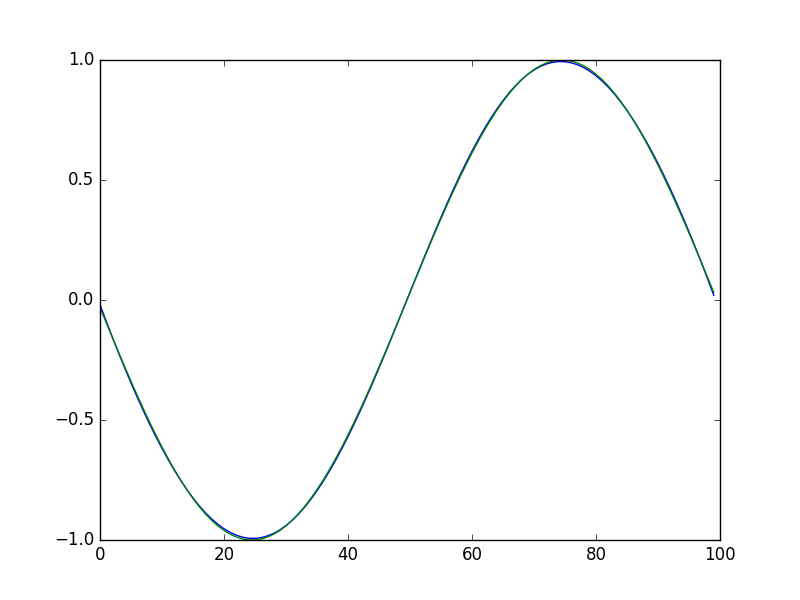
\includegraphics[width=.8\linewidth]{../fig2}
	\caption{最佳拟合(测试集)}
	\label{fig:fig2}
\end{figure}

由图\ref{fig:loss}可以看出,惩罚基本一直处于下降阶段,当学习达到第一个阶梯(1/3处),学习率下降时,惩罚也同样下降很多
\begin{figure}[h]
	\centering
	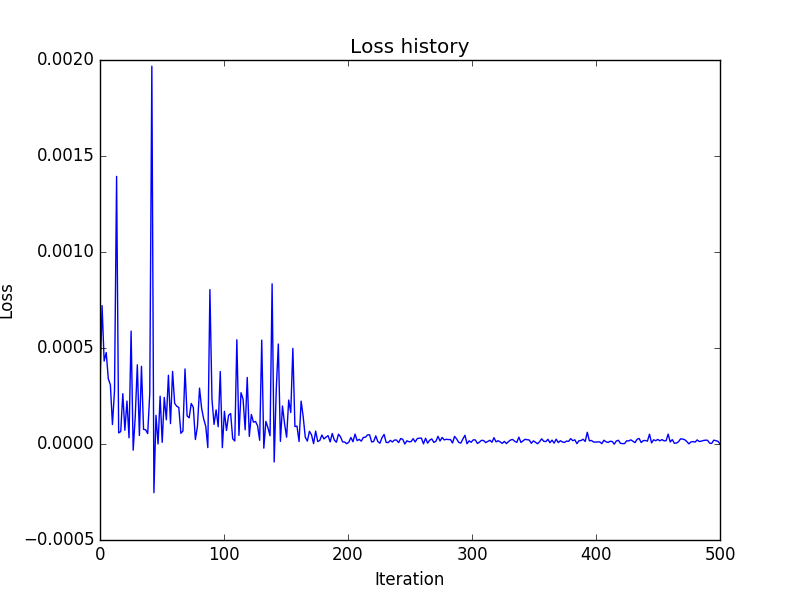
\includegraphics[width=.8\linewidth]{../loss}
	\caption{最佳拟合下的训练误差随时间变化图}
	\label{fig:loss}
\end{figure}

\section{实验总结}
通过上面分析可以看出,神经网络基本上能将函数$y=sin(x)$拟合出来。虽然BP神经网络具有较高的拟合能力,但是预测结果仍然存在一定的误差, 其拟合能力存在局限性。要想达到精确拟合,需要针对问题设计训练策略。
最终还要感谢相明老师的耐心指导。

{\small
	\bibliographystyle{ieee}
	\bibliography{he16sine}
}
\end{CJK}
\end{document}
